\section{Conclusion and Future Work}\label{sec:SurveyingConclusionFutureWork}
In this chapter we provided the details of how a swarm of RAVs can be used to gather data in a given region described by a polygon. We first described how to discretise the region into a set of grid points. We made some minor modifications to ensure that the implementation would be able to deal with real-world usage, which in practice takes the form of using the coordinate system that GPS depends on. We then implemented a Nearest Neighbor (NN) heuristic algorithm to generate routes for the swarm of RAVs which visit each grid point in the region exactly once, which is a solution to the multiple Travelling Salesman Problem. For practical purposes in relation to ROCSAFE \cite{Bagherzadeh2017ROCSAFE:Incidents}, the project that has funded this work, this offered a simple and scalable solution the surveying problem, but not a particularly efficient one. In order to run tests, we then used a web development framework to design a UI to interact with the grid generation code and the NN algorithm, which we used to generate some results which can be seen in tables \ref{table:NNAlgoResultsRect}, \ref{table:NNAlgoResultsTri}, \ref{table:NNAlgoResultsHex}, \ref{table:NNAlgoResultsIrregular}. Finally, we used the simulation environment, outlined in Chapter \ref{chap:HighFidelitySim}, to run further tests which offer highly realistic conditions, since the virtual RAVs run autopilot software that is used on real-world RAVs. These tests were carried out successfully and the results are illustrated in \ref{fig:VirtualPlannedRoutes}. 

We then began investigating using an optimisation tool to solve the more general problem of surveying with constrains such as heterogeneous RAV battery capacities, sampling times and operational speeds. We used the open-source Apache licensed Google OR-Tools repository to develop a prototype solution. This solution took orders of magnitude longer to calculate solutions compared to the NN algorithm, but offered qualitatively good solutions to the more general problem.



\subsubsection{Future Work}
Since we were limited by time constraints with this work, we outline some future work that we planned but did not have the time to execute. The points outlined are all taken to be specific to the Euclidean grid-based approach that was discussed throughout this chapter.

\begin{enumerate}

    \item A major limitation to the work done in this chapter is that we assume that RAVs act deterministically. In reality, there are many sources of randomness in environments that RAVs operate in. An approach that can deal with this randomness would have a major advantage over any approach that assumes determinism.
    
    \item Our approach is centralised, which means that RAVs do not act as independent agents. If for some reason an agent failed or communications were lost between RAVs and the central controller, the system would fail catastrophically. Future work could focus on modifying the approach taken in this thesis which could allow the RAVs to negotiate on what work they do based on their capabilities. Re-negotiation could periodically occur in the case that a RAV is left idle when it could be participating in the task.
    
    %\item The quality of the solution to the TSP given by the NN algorithm is known to be dependent on the start position <suitable reference missing>. A common improvement to the algorithm is to run it $n$ times for each possible starting point at each node in the network of $n$ nodes, and then take the best solution found. In the case of the mTSP, for $k$ RAVs, this would mean exploring ${n \choose k}$ different combinations of starting positions, which may make the running time of the algorithm prohibitively long. Therefore, future research could explore an effective way of determining the best starting nodes for the RAVs without implementing a brute force search to improve the NN solution.
    %\item Many solutions to the mTSP problem use \textit{iterative improvement} strategies,  which use an existing algorithm to create a solution, then have another algorithm improve the solution.\textit{ Ensemble} strategies are also frequently used, which applies a set of algorithms to the  problem and returns the best solution. The use of either of these techniques with the NN algorithm could provide significantly better results, especially given that this has been shown in the case of Euclidean distance cost functions. For example, reversing some segments that "cross" guarantees an improvement via the \textit{triangle inequality}, as shown in Figure \ref{fig:fixingTourCrossing}. 
    %\item Many open-source and commercial linear program solvers exist which are optimized to deal with the mTSP and VRP. We discussed how we used Google's OR-Tools repository <link in footnote> to prototype a solution. Future work could involve optimising the configuration of the problem and choice of back-end solver to produce a scalable solution.
    \item Representing the problem in a different manner may yield a suitable solution that is easier to computer. For example, representing the region to survey as continuous space rather than a discrete grid may facilitate the development of a control algorithm that is simpler and more effective in solving the surveying problem than the ones that exist that deal with discrete grids.
    \item Theoretical analysis of the performing surveying tasks with a swarm of RAVs may yield some insight into how to create a scalable algorithm for certain classes of grid (e.g. some regular shapes or compositions of regular shapes).
    \item The surveying task can be used to provide data to other algorithms that can provide useful tools when managing a disaster scene. For example, \textit{structure-from-motion} is a well-known technique for creating three-dimensional point clouds from two-dimensional images. A review of techniques used for structure-from-motion can be found in \cite{Bianco2018EvaluatingPipelines}. There may be potential to perform optimisations in the generation of the spacing and altitude of the grid points as well as the sequence in which the points are collected in order to generate the most accurate point cloud possible. We use the sample data collected as prior information for the stochastic target localisation problem outlined in Chapter \ref{chap:targetLocalisation}
    
    
\end{enumerate}


%\begin{figure}
%\centering
%\begin{minipage}{.5\textwidth}
%  \centering
%  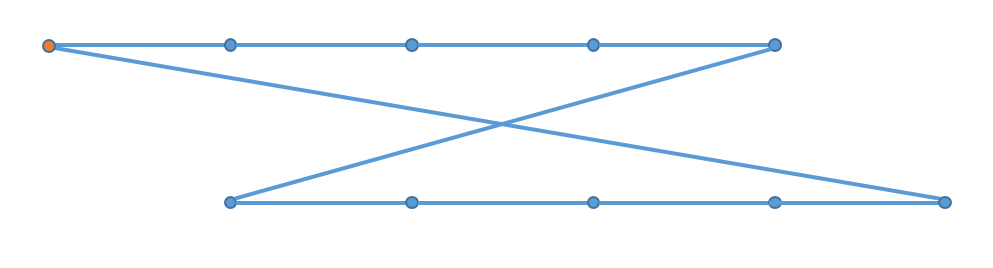
\includegraphics[width=.48\linewidth]{Chapters/MultiAgentCoverage/Figs/crossingSegments.PNG}
%  \captionof*{figure}{"X" present in a tour}
%  \label{fig:crossingTour}
%\end{minipage}%
%\begin{minipage}{.5\textwidth}
%  \centering
%  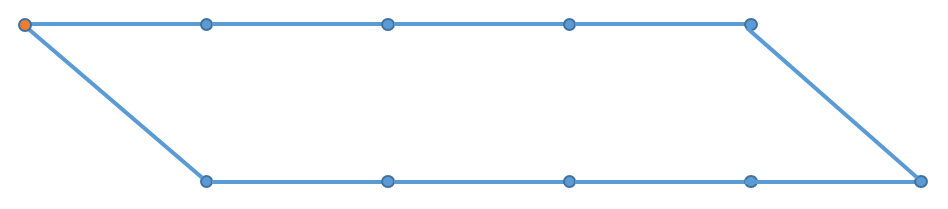
\includegraphics[width=.48\linewidth]{Chapters/MultiAgentCoverage/Figs/nonCrossingSegments.png}
%  \captionof*{figure}{"X" removed from tour by reversing segments}
%  \label{fig:nonCrossingTour}
%\end{minipage}
%\caption{Using the triangle inequality to improve tours.}
%Figures based on those found in \href{https://github.com/norvig/pytudes/blob/master/ipynb/TSP.ipynb}{Norvig's TSP github repo.}}
%\footnote{\href {https://github.com/norvig/pytudes/blob/master/ipynb/TSP.ipynb}{https://github.com/norvig/pytudes/blob/master/ipynb/TSP.ipynb}}
%\label{fig:fixingTourCrossing}
%\end{figure}
%\footnote{\href {https://github.com/norvig/pytudes/blob/master/ipynb/TSP.ipynb}{https://github.com/norvig/pytudes/blob/master/ipynb/TSP.ipynb}}























